%definira klasu dokumenta 
\documentclass[12pt]{report} 

%prostor izmedu naredbi \documentclass i \begin{document} se zove uvod. U njemu se nalaze naredbe koje se odnose na cijeli dokument

%osnovni LaTex ne može riješiti sve probleme, pa se koriste različiti paketi koji olakšavaju izradu željenog dokumenta
\usepackage[croatian]{babel} 
\usepackage{amssymb}
\usepackage{amsmath}
\usepackage{txfonts}
\usepackage{mathdots}
\usepackage{titlesec}
\usepackage{array}
\usepackage{lastpage}
\usepackage{etoolbox}
\usepackage{tabularray}
\usepackage{color, colortbl}
\usepackage{adjustbox}
\usepackage{geometry}
\usepackage[classicReIm]{kpfonts}
\usepackage{hyperref}
\usepackage{fancyhdr}

\usepackage{float}
\usepackage{setspace}
\restylefloat{table}


\patchcmd{\chapter}{\thispagestyle{plain}}{\thispagestyle{fancy}}{}{} %redefiniranje stila stranice u paketu fancyhdr

%oblik naslova poglavlja
\titleformat{\chapter}{\normalfont\huge\bfseries}{\thechapter.}{20pt}{\Huge}
\titlespacing{\chapter}{0pt}{0pt}{40pt}


\linespread{1.3} %razmak između redaka

\geometry{a4paper, left=1in, top=1in,}  %oblik stranice

\hypersetup{ colorlinks, citecolor=black, filecolor=black, linkcolor=black,	urlcolor=black }   %izgled poveznice


%prored smanjen između redaka u nabrajanjima i popisima
\newenvironment{packed_enum}{
	\begin{enumerate}
		\setlength{\itemsep}{0pt}
		\setlength{\parskip}{0pt}
		\setlength{\parsep}{0pt}
	}{\end{enumerate}}

\newenvironment{packed_item}{
	\begin{itemize}
		\setlength{\itemsep}{0pt}
		\setlength{\parskip}{0pt}
		\setlength{\parsep}{0pt}
	}{\end{itemize}}




%boja za privatni i udaljeni kljuc u tablicama
\definecolor{LightBlue}{rgb}{0.9,0.9,1}
\definecolor{LightGreen}{rgb}{0.9,1,0.9}

%Promjena teksta za dugačke tablice
\DefTblrTemplate{contfoot-text}{normal}{Nastavljeno na idućoj stranici}
\SetTblrTemplate{contfoot-text}{normal}
\DefTblrTemplate{conthead-text}{normal}{(Nastavljeno)}
\SetTblrTemplate{conthead-text}{normal}
\DefTblrTemplate{middlehead,lasthead}{normal}{Nastavljeno od prethodne stranice}
\SetTblrTemplate{middlehead,lasthead}{normal}

%podesavanje zaglavlja i podnožja

\pagestyle{fancy}
\lhead{Programsko inženjerstvo}
\rhead{$Sinappsa$}
\lfoot{$TurbulenTech$}
\cfoot{stranica \thepage/\pageref{LastPage}}
\rfoot{\today}
\renewcommand{\headrulewidth}{0.2pt}
\renewcommand{\footrulewidth}{0.2pt}


\begin{document} 
	
	
	
	\begin{titlepage}
		\begin{center}
			\vspace*{\stretch{1.0}} %u kombinaciji s ostalim \vspace naredbama definira razmak između redaka teksta
			\LARGE Programsko inženjerstvo\\
			\large Ak. god. 2022./2023.\\
			
			\vspace*{\stretch{3.0}}
			
			\huge $Sinappsa$\\
			\Large Dokumentacija, Rev. \textit{$ 1 $}\\
			
			\vspace*{\stretch{12.0}}
			\normalsize
			Grupa: \textit{$TurbulentTech$}\\
			Voditelj: \textit{$Mislav$ $Đomlija$}\\
			
			
			\vspace*{\stretch{1.0}}
			Datum predaje: \textit{$17$. $studenog$ $2022$.}\\
	
			\vspace*{\stretch{4.0}}
			
			Nastavnik: \textit{$Laura$ $Majer$}\\
		
		\end{center}

	
	\end{titlepage}

	
	\tableofcontents


	\chapter{Dnevnik promjena dokumentacije}
		
		
		
		\begin{longtblr}[
				label=none
			]{
				width = \textwidth, 
				colspec={|X[2]|X[13]|X[3]|X[3]|}, 
				rowhead = 1
			}
			\hline
			\textbf{Rev.}	& \textbf{Opis promjene/dodatka} & \textbf{Autori} & \textbf{Datum}\\[3pt] \hline
			0.1 & Napravljen predložak.	& Mislav Đomlija & 3.11.2022. 		\\[3pt] \hline 
			0.2	& Dopisane upute za povijest dokumentacije.\newline Dodane reference. & * & 24.08.2013. 	\\[3pt] \hline 
			0.5 & Dodan \textit{Use Case} dijagram i jedan sekvencijski dijagram, funkcionalni i nefunkcionalni zahtjevi i dodatak A & Maksim Kos & 12.11.2022. \\[3pt] \hline 
			0.6 & Arhitektura i dizajn sustava, algoritmi i strukture podataka & * & 26.08.2013. \\[3pt] \hline 
			0.8 & Povijest rada i trenutni status implementacije,\newline Zaključci i plan daljnjeg rada & * & 28.08.2013. \\[3pt] \hline 
			0.9 & Opisi obrazaca uporabe & Maksim Kos & 07.11.2022. \\[3pt] \hline 
			0.10 & Preveden uvod &Maksim Kos& 12.11.2022. \\[3pt] \hline 
			0.11 & Sekvencijski dijagrami & Maksim Kos& 07.11.2022. \\[3pt] \hline 
			0.12.1 & Započeo dijagrame razreda & * & 10.09.2013. \\[3pt] \hline 
			0.12.2 & Nastavak dijagrama razreda & * & 11.09.2013. \\[3pt] \hline 
			\textbf{1.0} & Verzija samo s bitnim dijelovima za 1. ciklus & * & 11.09.2013. \\[3pt] \hline 
			1.1 & Uređivanje teksta -- funkcionalni i nefunkcionalni zahtjevi & * \newline * & 14.09.2013. \\[3pt] \hline 
			1.2 & Manje izmjene:Timer - Brojilo vremena & * & 15.09.2013. \\[3pt] \hline 
			1.3 & Popravljeni dijagrami obrazaca uporabe & * & 15.09.2013. \\[3pt] \hline 
			1.5 & Generalna revizija strukture dokumenta & * & 19.09.2013. \\[3pt] \hline 
			1.5.1 & Manja revizija (dijagram razmještaja) & * & 20.09.2013. \\[3pt] \hline 
			\textbf{2.0} & Konačni tekst predloška dokumentacije  & * & 28.09.2013. \\[3pt] \hline 
			&  &  & \\[3pt] \hline	
		\end{longtblr}
	
	
		\textit{Moraju postojati glavne revizije dokumenata 1.0 i 2.0 na kraju prvog i drugog ciklusa. Između tih revizija mogu postojati manje revizije već prema tome kako se dokument bude nadopunjavao. Očekuje se da nakon svake značajnije promjene (dodatka, izmjene, uklanjanja dijelova teksta i popratnih grafičkih sadržaja) dokumenta se to zabilježi kao revizija. Npr., revizije unutar prvog ciklusa će imati oznake 0.1, 0.2, …, 0.9, 0.10, 0.11.. sve do konačne revizije prvog ciklusa 1.0. U drugom ciklusu se nastavlja s revizijama 1.1, 1.2, itd.}
	\chapter{Opis projektnog zadatka}
		
		\textbf{\textit{dio 1. revizije}}\\
		
		{Cilj ovog projekta je razviti programsku potporu za stvaranje web aplikacije \textit{"Sinappsa"} koja će omogućiti korisniku prvenstveno studentima Fakulteta Elektrotehnike i Računastva da ponude pomoć ili zatraže pomoć oko specifičnog gradiva, labaratorijske vježbe, ispita ili kolegija općenito. Također aplikacija će održavati i rejting listu najuspješnijih studenata-pomagača. Tako će korisnicima biti lakše tražiti ili nuditi pomoć te biti u mogućnosti odabrati što boljeg studenta-pomagača.
		\\
		\indent Prilikom pokretanja sustava prikazuje se lista najnovijih objavljenih oglasa te rejting lista najbolje recenziranih studenata pomagača
		\\
		\indent Neregistriranom korisniku dostupna je lista trenutno objavljenih oglasa kao i rejting-lista studenta-pomagača. Neregistrirani korisnik može oglase filtrirati po smjeru(računastvo ili elektrotehnika), kolegiju(ViS, UPRO, ARH2, PPJ, UTR) i kategoriji(labaratorijska vježba, blic, zadaća, ispitni rok). Neregistriranom korisniku nije moguće kontaktiranje davatelja oglasa odnosno odgovaranje na oglas. Neregistriranom korisniku omogućeno je prijavljivanje u sustav s postojećim računom(potrebno je upisati korisničko ime i lozinku) ili kreirati novi račun(kojim će postati registrirani korisnik). Prilikom kreiranja novog računa potreban je unos sljedećih podataka: 
		\begin{packed_item}
			
			\item  ime
			\item  prezime
			\item  korisničko ime
			\item  lozinka
			\item  email adresa

		\end{packed_item}
		\indent Registracijom u sustav koriniku se dodjeljuju prava koja ima registrirani korisnik. Registriranom korisniku mogu biti i dodjeljena prava moderatora. Registrirani korisnik može kao i neregistrirani korisnik pregledavati oglasi te uz to objavljivati i odgovarati na oglase.\\
		\indent \underbar{Moderator} može uz sva prava registriranog korisnika uklanjati nepravilne ili neprikladne oglase. 
		}
		
		
	
	\chapter{Specifikacija programske potpore}
		
	\section{Funkcionalni zahtjevi}
			
			\textbf{\textit{dio 1. revizije}}\\
			
			\textit{Navesti \textbf{dionike} koji imaju \textbf{interes u ovom sustavu} ili  \textbf{su nositelji odgovornosti}. To su prije svega korisnici, ali i administratori sustava, naručitelji, razvojni tim.}\\
				
			\textit{Navesti \textbf{aktore} koji izravno \textbf{koriste} ili \textbf{komuniciraju sa sustavom}. Oni mogu imati inicijatorsku ulogu, tj. započinju određene procese u sustavu ili samo sudioničku ulogu, tj. obavljaju određeni posao. Za svakog aktora navesti funkcionalne zahtjeve koji se na njega odnose.}\\
			
			
			\noindent \textbf{Dionici:}
			
			\begin{packed_enum}
				\item Naručitelj
				\item Studenti 
				    \begin{packed_enum}
				        \item Pomagač
				        \item Traži pomoć
				    \end{packed_enum}
				\item Administrator
				\item Razvojni tim
				
			\end{packed_enum}
			
			\noindent \textbf{Aktori i njihovi funkcionalni zahtjevi:}
			
			
			\begin{packed_enum}
				\item  \underbar{Neregistrirani korisnik (inicijator) može:}
				
				\begin{packed_enum}
					
					\item pregledati listu trenutno objavljenih oglasa
					\item pregledati rejting listu studenata-pomagača
					\item filtirati oglase po smjeru, kolegiju i kategoriji
					\item se registrirati u sustav, stvoriti novi korisnicki račun za koji su mu potrebni korisničko ime, lozinka, ime, prezime, e-mail adresa i opcionalno profila slika
					
				\end{packed_enum}
			
				\item  \underbar{Registrirani korisnik (inicijator) može:}
				
				\begin{packed_enum}
					
					\item pregledati listu trenutno objavljenih oglasa
					\item pregledati rejting listu studenata-pomagača
					\item filtirati oglase po smjeru, kolegiju i kategoriji
					\item može objavljivati i odgovarati na oglase
					\item može pregledavati svoje aktivne i neaktivne oglase
					\item može uređivati ili obrisati vlastite oglase
					\item može pregledavati sve svoje trenutne upite
					\item može davati ocjenu studetnu-pomagaču
					\item može promjeniti profilnu, lozinku ili korisničko ime
					\item može izbrisati korisnički račun
					
				\end{packed_enum}
				
				\item  \underbar{Moderator (inicijator) može:}
				
				\begin{packed_enum}
					
					\item pregledati listu trenutno objavljenih oglasa
					\item pregledati rejting listu studenata-pomagača
					\item filtirati oglase po smjeru, kolegiju i kategoriji
					\item može objavljivati i odgovarati na oglase
					\item može pregledavati svoje aktivne i neaktivne oglase
					\item može uređivati ili obrisati vlastite oglase
					\item može pregledavati sve svoje trenutne upite
					\item može davati ocjenu studetnu-pomagaču
					\item može promjeniti profilnu, lozinku ili korisničko ime
					\item može izbrisati korisnički račun
					\item može brisati tuđe oglase uz dani razlog
					
				\end{packed_enum}
				
				\item  \underbar{Registrirani korisnik (inicijator) može:}
				
				\begin{packed_enum}
					
					\item pregledati listu trenutno objavljenih oglasa
					\item pregledati rejting listu studenata-pomagača
					\item filtirati oglase po smjeru, kolegiju i kategoriji
					\item može objavljivati i odgovarati na oglase
					\item može pregledavati svoje aktivne i neaktivne oglase
					\item može uređivati ili obrisati vlastite oglase
					\item može pregledavati sve svoje trenutne upite
					\item može davati ocjenu studetnu-pomagaču
					\item može promjeniti profilnu, lozinku ili korisničko ime
					\item može izbrisati korisnički račun
					
				\end{packed_enum}
				
				\item  \underbar{Baza podataka (sudionik) može:}
				
				\begin{packed_enum}
					
					\item pohranjuje sve podatke o korisnicima i njihovim ovlastima
					\item pohranjuje sve podatke o oglasima i upitima
					\item pohranjuje sve obrisane oglase (neprikladne ili obrisane od strane korisnika)
					
				\end{packed_enum}
				
				
			\end{packed_enum}
			
			\eject 
			
			
				
			\subsection{Obrasci uporabe}
				
		
					\noindent \underbar{\textbf{UC1 -Registracija}}
					\begin{packed_item}
	
						\item \textbf{Glavni sudionik: }Korisnik
						\item  \textbf{Cilj:} Stvaranje korisničkog računa 
						\item  \textbf{Sudionici:} Baza podataka
						\item  \textbf{Preduvjet:} -
						\item  \textbf{Opis osnovnog tijeka:}
						
						\item[] \begin{packed_enum}
	
							\item Neregistrirani korisnik odabire opciju za registraciju
							\item Neregistrirani korisnik unosi potrebne korisničke podatke
							\item Korisnik prima obavijest o uspješnoj registraciji
						\end{packed_enum}
						
						\item  \textbf{Opis mogućih odstupanja:}
						
						\item[] \begin{packed_item}
	
							\item[2.a] Odabir već zauzetog korisničkog imena ili neispravnog e-mail adrese, unos korisničkog podatka u nedozvoljenom formatu
							\item[] \begin{packed_enum}
								
								\item Sustav obavještava korisnika o neuspjelom upisu i vraća ga na stranicu za registraciju
								\item Korisnik mijenja potrebne podatke te završava unos ili odustaje od registracije
								
							\end{packed_enum}
						\end{packed_item}
					\end{packed_item}
					
					\noindent \underbar{\textbf{UC2 -Prijava u sustav}}
					\begin{packed_item}
	
						\item \textbf{Glavni sudionik: }Korisnik
						\item  \textbf{Cilj:} Dobiti mogućnosti interakcija s oglasima(objavljivanje, brisanje ili slanje upita)
						\item  \textbf{Sudionici:} Baza podataka
						\item  \textbf{Preduvjet:} Registracija
						\item  \textbf{Opis osnovnog tijeka:}
						
						\item[] \begin{packed_enum}
	
							\item Unos korisničkog imena i lozinke
							\item Potvrda o ispravnosti unesenih podataka
							\item Pristup korisničkim funckijama
							
						\end{packed_enum}
						
						\item  \textbf{Opis mogućih odstupanja:}
						
						\item[] \begin{packed_item}
	
							\item[2.a] Neispravno korisničko ime/lozinka
							\item[] \begin{packed_enum}
								
								\item Sustav obaviještava korisnika o neuspjelom upisu i vraća ga na stranicu za prijavu u aplikaciju

								
							\end{packed_enum}
						\end{packed_item}
					\end{packed_item}
					
					\noindent \underbar{\textbf{UC3 -Pregled oglasa}}
					\begin{packed_item}
	
						\item \textbf{Glavni sudionik: }Korisnik
						\item  \textbf{Cilj:} Pregled aktivnih oglasa
						\item  \textbf{Sudionici:} Baza podataka
						\item  \textbf{Preduvjet:} -
						\item  \textbf{Opis osnovnog tijeka:}
						
						\item[] \begin{packed_enum}
	
							\item Lista svih aktivnih oglasa je prikazana pilikom učitavanja aplikacije
							\item Mogućnost filtriranja oglasa po određenim kriterijima
							\item $<$opis korak tri$>$
							\item $<$opis korak četiri$>$
							\item $<$opis korak pet$>$
						\end{packed_enum}

					\end{packed_item}
					
					\noindent \underbar{\textbf{UC4 -Pretraga oglasa}}
					\begin{packed_item}
	
						\item \textbf{Glavni sudionik: }Korisnik
						\item  \textbf{Cilj:} Filtrirati oglase po vlastitim kriterijima
						\item  \textbf{Sudionici:} Baza podataka
						\item  \textbf{Preduvjet:} -
						\item  \textbf{Opis osnovnog tijeka:}
						
						\item[] \begin{packed_enum}
	
							\item Korisnik filtrira oglase po kriteriju kolegija, smjera i kategorije
							\item Izlistaju se oglasi koji zadovoljavaju tražene kriterije
						\end{packed_enum}
						
						\item  \textbf{Opis mogućih odstupanja:}
						
						\item[] \begin{packed_item}
	
							\item[2.a] Niti jedan oglas ne zadovoljava tražene kriterije
							\item[] \begin{packed_enum}
								
								\item Korisnika se obaviještava da nema traženog oglasa
								
							\end{packed_enum}

							
						\end{packed_item}
					\end{packed_item}
					
					\noindent \underbar{\textbf{UC5 -Uređivanje vlastitih oglasa}}
					\begin{packed_item}
	
						\item \textbf{Glavni sudionik: } Korisnik
						\item  \textbf{Cilj:} Preudrediti objavljeni oglas
						\item  \textbf{Sudionici:} Baza podataka
						\item  \textbf{Preduvjet:} 
						    \begin{packed_enum}
	
							\item Korisnik je prijavljen u sustav
							\item Oglas je aktivan
						    \end{packed_enum}
						\item  \textbf{Opis osnovnog tijeka:}
						
						\item[] \begin{packed_enum}
	
							\item Korisnik odabire opcije preuredi
							\item Preuređuje naslov/opis oglasa
							\item Odabire opciju pohrani
							\item Promjene se pohranjuju u bazu podataka
						\end{packed_enum}
						
					
					\end{packed_item}
					
					\noindent \underbar{\textbf{UC6 -Reply na oglas}}
					\begin{packed_item}
	
						\item \textbf{Glavni sudionik: } Korisnik
						\item  \textbf{Cilj:} Postaviti upit na oglas
						\item  \textbf{Sudionici:} Baza podataka
						\item  \textbf{Preduvjet:} 
						    \begin{packed_enum}
	
							\item Korisnik je prijavljen u sustav
							\item Oglas je aktivan
						    \end{packed_enum}
						\item  \textbf{Opis osnovnog tijeka:}
						
						\item[] \begin{packed_enum}
	
							\item Korisnik odabire opciju reply
							\item Korisnik unosi traženu poruku
							\item Korisniku koji je objavio oglas se šalje e-mail s upitom i kontakt podatcima zainteresiranog korisnika
							\item Upit se pohranjuje u bazu podataka
						\end{packed_enum}
						
					
					\end{packed_item}
					
					\noindent \underbar{\textbf{UC7 -Post oglas}}
					\begin{packed_item}
	
						\item \textbf{Glavni sudionik: } Korisnik
						\item  \textbf{Cilj:} Objaviti oglas
						\item  \textbf{Sudionici:} Baza podataka
						\item  \textbf{Preduvjet:} Korisnik je prijavljen u sustav

						\item  \textbf{Opis osnovnog tijeka:}
						
						\item[] \begin{packed_enum}
	
							\item Korisnik odabire opciju post 
							\item Korisnik unosi traženi naslov, opis,kolegij i kategoriju
							\item Oglas se pohranjuje u bazu podataka
						\end{packed_enum}
						
					
					\end{packed_item}
					
					\noindent \underbar{\textbf{UC8 -Ocjenjivanje studenta-pomagača}}
					\begin{packed_item}
	
						\item \textbf{Glavni sudionik: } Korisnik
						\item  \textbf{Cilj:} Ocjeniti studenta-pomagača
						\item  \textbf{Sudionici:} Baza podataka
						\item  \textbf{Preduvjet:} 
						    \begin{packed_enum}
	
							\item Korisnik je prijavljen u sustav
							\item Oglas je aktivan
							\item Oglas je tipa \textit{nudim}
							\item Reply je statusa \textit{prihvaćen}
						    \end{packed_enum}
						\item  \textbf{Opis osnovnog tijeka:}
						
						\item[] \begin{packed_enum}
	
							\item Korisnik odabire opciju ocjeni
							\item Korisnik unosi ocjenu izvrsnosti studenta-pomagača
							\item Ocjena se pribraja u dosadašnje ocjene studenta-pomagača
							\item Ocjena se pohranjuje u bazu podataka
						\end{packed_enum}
						
						\item  \textbf{Opis mogućih odstupanja:}
						
						\item[] \begin{packed_item}
	
							\item[2.a] Oglas je izbrisan
							\item[] \begin{packed_enum}
								
								\item Korisnika se obaviještava da nema mogućnost ocjene studenta-pomagača
								
							\end{packed_enum}

							
						\end{packed_item}
						
					
					\end{packed_item}
					
					\noindent \underbar{\textbf{UC9 -Pregled osobnih podataka}}
					\begin{packed_item}
	
						\item \textbf{Glavni sudionik: }Korisnik
						\item  \textbf{Cilj:} Pregledati osobne podatke
						\item  \textbf{Sudionici:} Baza podataka
						\item  \textbf{Preduvjet:} Klijent prijavljen u sustav
						\item  \textbf{Opis osnovnog tijeka:}
						
						\item[] \begin{packed_enum}
	
							\item Korisnik odabire opciju "Osobni podatci"
							\item Aplikacija prikazuje osobne podatke korisnika
						\end{packed_enum}
						
					\end{packed_item}
					
					
					
					
						\noindent \underbar{\textbf{UC10 -Promjena osobnih podataka}}
					\begin{packed_item}
	
						\item \textbf{Glavni sudionik: }Korisnik
						\item  \textbf{Cilj:} Promijeniti osobne podatke
						\item  \textbf{Sudionici:} Baza podataka
						\item  \textbf{Preduvjet:} Korisnik je prijavljen
						\item  \textbf{Opis osnovnog tijeka:}
						
						\item[] \begin{packed_enum}
	
							\item Korisnik odabere opciju za promjenu podataka
							\item Korisnik mijenja svoje osobne podatke
							\item Korisnik sprema promjene
							\item Baza podataka se ažurira

						\end{packed_enum}
						
						\item  \textbf{Opis mogućih odstupanja:}
						
						\item[] \begin{packed_item}
	
							\item[2.a] Korisnik promijeni svoje osobne podatke, ali ne odabere opciju "Spremi promjenu"
							\item[] \begin{packed_enum}
								
								\item Sustav obavještava korisnika da nije spremio podatke prije izlaska iz prozora
								
							\end{packed_enum}
							\item[2.b] Korisnik unosi već zauzeto korisničko ime
                            \item[] \begin{packed_enum}
								
								\item Sustav obavještava korisnika da je unio već zauzeto korisničko ime
								
							\end{packed_enum}
							
						\end{packed_item}
					\end{packed_item}
					
					\noindent \underbar{\textbf{UC11 -Brisanje korisničkog računa}}
					\begin{packed_item}
	
						\item \textbf{Glavni sudionik: }Korisnik
						\item  \textbf{Cilj:} zbrisati svoj korisnički račun
						\item  \textbf{Sudionici:} Baza podataka
						\item  \textbf{Preduvjet:} Korisnik je prijavljen
						\item  \textbf{Opis osnovnog tijeka:}
						
						\item[] \begin{packed_enum}
	
							\item  Korisnik pregledava osobne podatke
							\item Otvara se stranica s osobnim podacima korisnika
							\item Korisnik briše račun
							\item Korisnički račun se izbriše iz baze podataka
							\item Otvara se početna stranica
						\end{packed_enum}
					
					\end{packed_item}
					
					
                
                    \noindent \underbar{\textbf{UC12 -Brisanje oglasa}}
					\begin{packed_item}
	
						\item \textbf{Glavni sudionik: }Moderator
						\item  \textbf{Cilj:} Ukloniti neprikladne oglase
						\item  \textbf{Sudionici:} Baza podataka
						\item  \textbf{Preduvjet:} Korisnik ima ulogu moderatora
						\item  \textbf{Opis osnovnog tijeka:}
						
						\item[] \begin{packed_enum}
	
							\item Moderator primjećuje da je određenih aktivni oglas neprikladan
							\item Odabire opciju obriši te daje objašnjenje kreatoru oglasa
							\item Kreator oglasa je obaviješten putem e-mail adrese o uklanjaju oglasa
						\end{packed_enum}
						
						\item  \textbf{Opis mogućih odstupanja:}
						
						\item[] \begin{packed_item}
	
							\item[2.a] Oglas je već uklonjen ili obrisan od strane kreatora, ali je idalje vidljiv u aplikaciji
							\item[] \begin{packed_enum}
								
								\item Obavijest moderatoru da je dani oglas uklonjen

								
							\end{packed_enum}
						\end{packed_item}
					\end{packed_item}				
				
			\eject	
			\begin{fig}
			    \subsubsection{Dijagrami obrazaca uporabe}
			    
                    \graphicspath{ {slike/} }
  
                    \centering
                    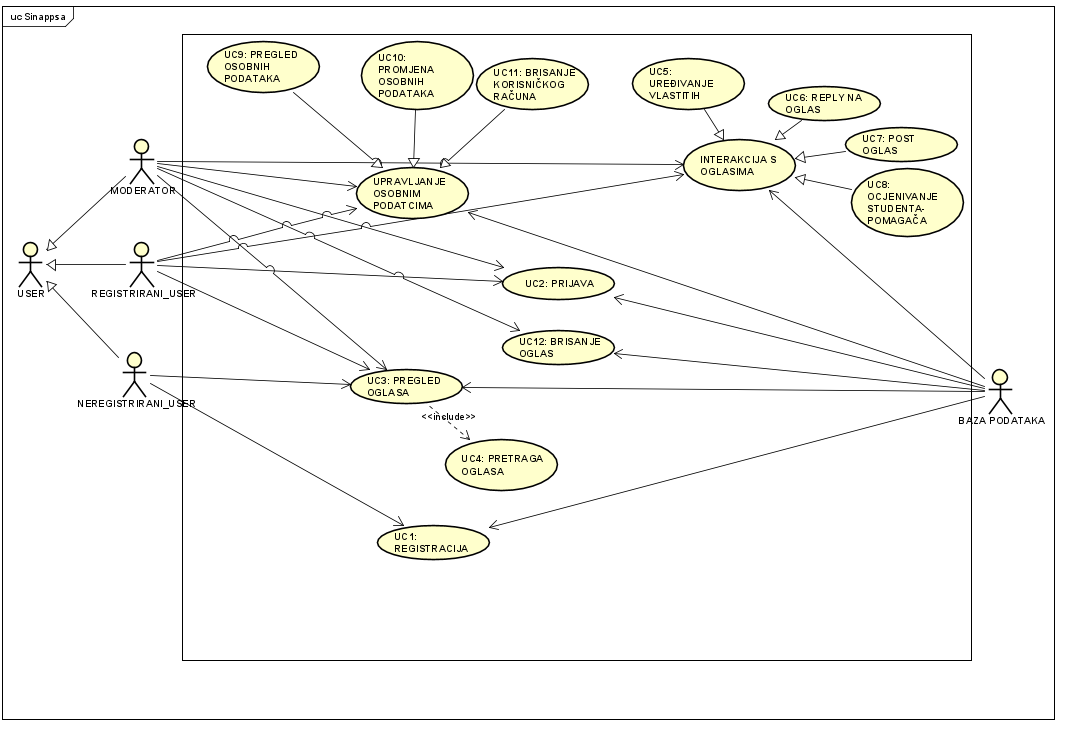
\includegraphics[width=\textwidth]{UseCase-slika.png}
                    \caption{\Slika 3.1: Dijagram obrasca uporabe registrirano korisnika, neregistriranog korisnika, moderatora i baze podataka}
               
			\eject	
			
			\end{fig}
				

			
			\subsection{Sekvencijski dijagrami}
				
				
				\noindent\textbf{Obrazac uporabe UC1-Registracija}\\
				Neregistrirani korisnik zatraži stranicu za registraciju kako bi se registirao i imao mogućnosti koje ima registrirani korisnik. Web-aplikacija mu prikazuje stranicu za registraciju. Korisnik unosi sve potrebne podatke za registraciju koje web-aplikacija zaprima i provjerava unikatnost unesenih podataka s bazom podataka točnije unikatnost e-mail adrese i username-a. Sama web-aplikacija validira valjanost podataka te korisniku vraća rezultat uspješnosti registracije. ako je registracija neuspjela vraća ga na početnu formu za registraciju. Korisnik tokom registracijskog procesa može odustati od registracije te ga web-aplikacija vraća na početnu stranicu. Nakon uspješne registracije registriranog korisnika vraća na početnu stranicu. 
				\\
                \begin{fig}
				    \graphicspath{ {slike/} }
  
                    \centering
                    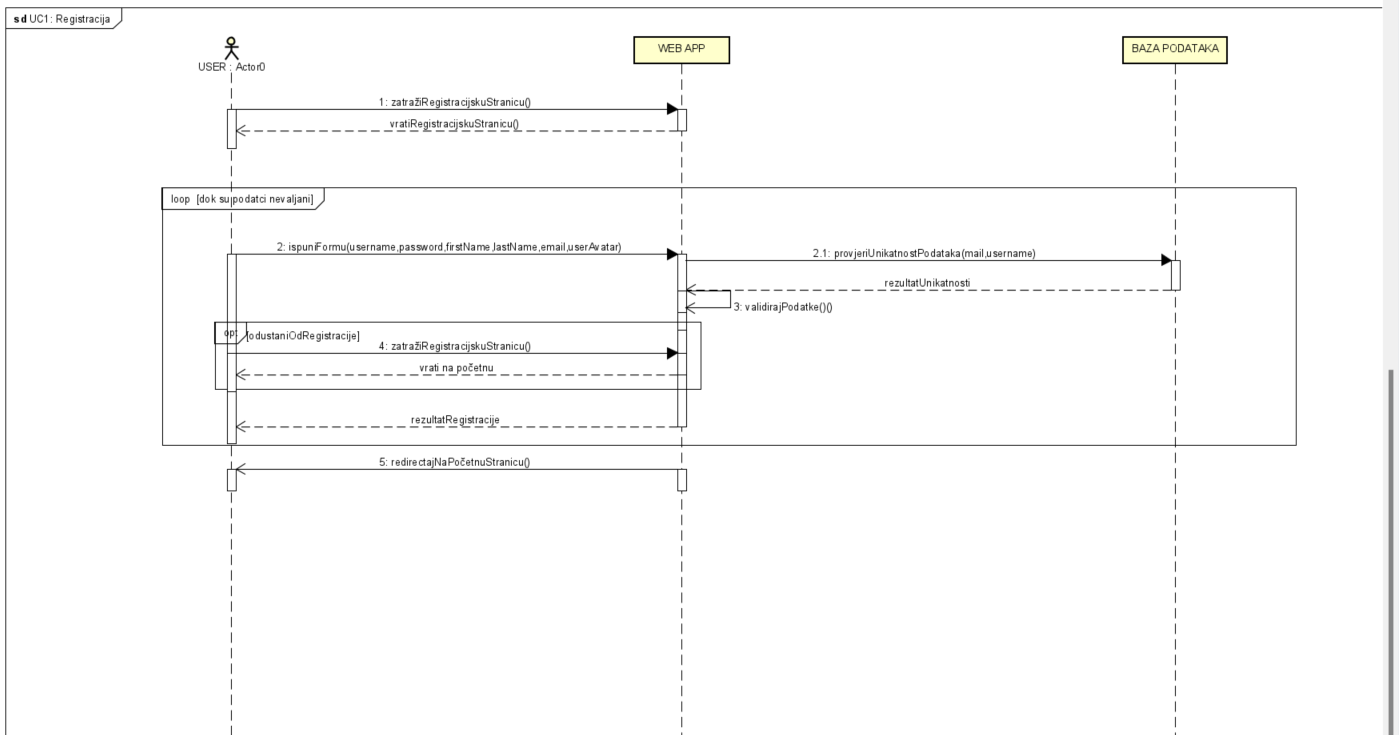
\includegraphics[width=\textwidth]{UC1_ Registracija_sekvencijskiDijagram.png}
                    \caption{\Slika 3.2: Sekvencijski dijagram za UC1}
                \end{fig}
				\\
				\\
			    \noindent\textbf{Obrazac uporabe UC6-Reply na oglas}\\
			    Korisnik koji želi postaviti upit na traženi oglas odabire opciju reply te mu web-stranica dostvlja formu za reply. Korisnik unosi proizvoljni tekst koji se predaje web-stranici, a web-stranica prosljeđuje bazi podataka kako bi baza pohranila zadani upit. Web-stranica nakon pohrane upit u bazu podatak traži od baze podatke podatke o kreatoru oglasa na koji je zadani upit postavljen kako bi kreatora oglasa putem maila obavijestila da je nekao napravio upit na njegov oglas. Web-stranica na kraju kreatoru upita daje doznanja da je mail poslan kreatoru oglasa.
			    \\
                \begin{fig}
				    \graphicspath{ {slike/} }
  
                    \centering
                    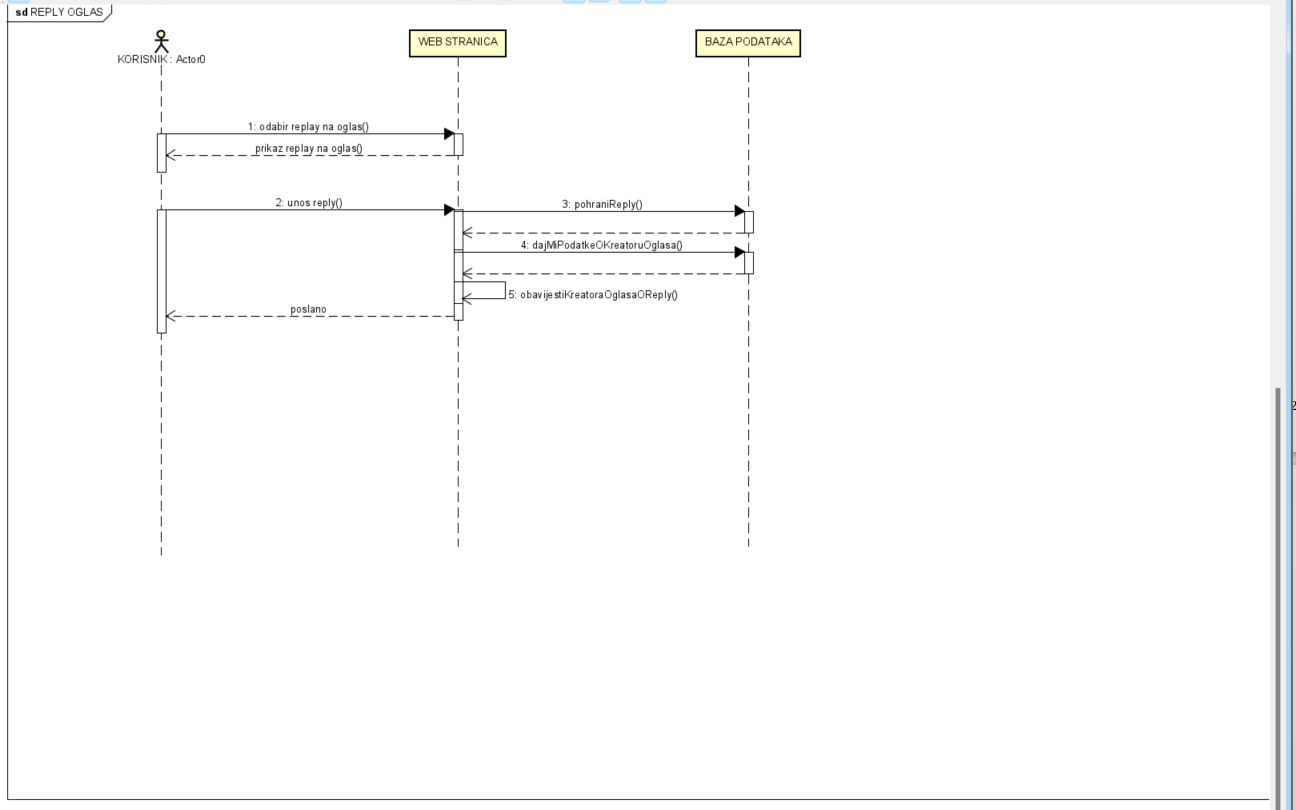
\includegraphics[width=\textwidth]{REPLY OGLAS.png}
                    \caption{\Slika 3.3: Sekvencijski dijagram za UC6}
                \end{fig}
				\\

			    \noindent\textbf{Obrazac uporabe UC7-Post oglas}\\
			    Korisnik želi objaviti oglas neovisno o samom tipu oglasa(dajem/nudim). Korisnik odabire opciju stvaranje novog oglasa te mu web-stranica vraća formu za stvaranje oglasa. Korsinik unosi podatke za oglas te unos predaje web-stranici koja provjerava valjanost unosa. Ako je unos nevaljan web-stranica vraća korisnika ponovno na formu za stvaranje oglasa ili korisnik odluči odustati od kreiranja oglasa te ga web-stranica vraća na početnu stranicu. Kada su uneseni podatci valjani korisnik objavljuje oglas te web-stranica oglas pohranjuje u bazu podataka. Na kraju web-stranica nakon uspješnog pohranjivanja oglasa u bazu podataka obaviještava korisnika da je oglas objavljen.
			    \\
			    \\
			    \begin{fig}
			   
				    \graphicspath{ {slike/} }
  
                    \centering
                    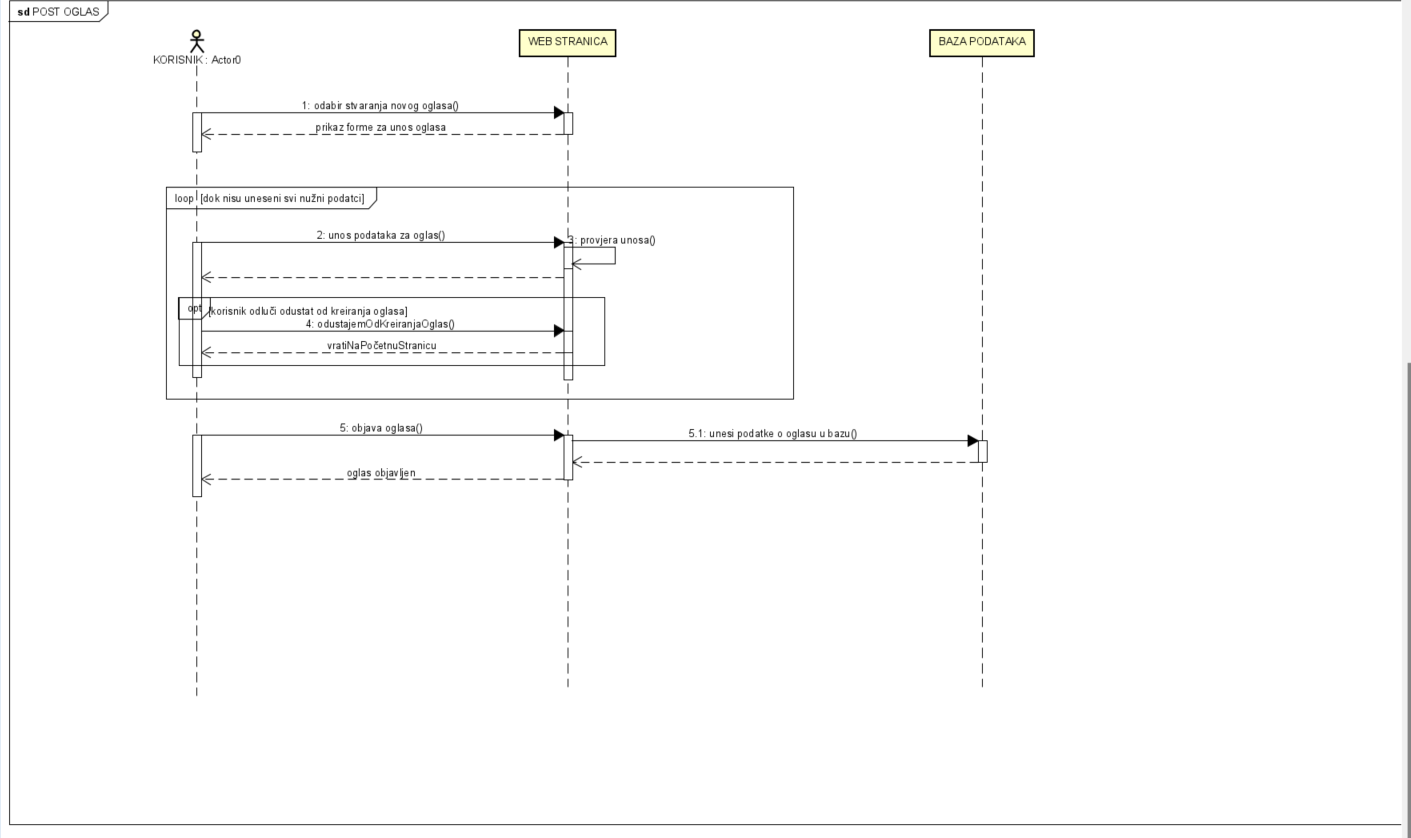
\includegraphics[width=\textwidth]{POST OGLAS.png}
                    \caption{\Slika 3.4: Sekvencijski dijagram za UC7}
                \end{fig}
			\eject

				\
	
		\section{Ostali zahtjevi}
		
			\textbf{\textit{dio 1. revizije}}\\
		 
			 \begin{packed_item}
	
			\item Sustav treba omogucitićiti rad višse korisnika u stvarnom vremenu
			\item  Korisničko sučelje i sustav moraju podržavati hrvatsku abecedu pri unosu i prikazu tekstualnog sadržaja 
			\item  Izvršavanje dijela programa u kojem se pristupa bazi podataka ne smije trajati duže od nekoliko sekundi
			\item  Sustav treba biti implementiran kao web aplikacija koristeci multiparadigmatski jezik
			\item  Sustav treba biti jednostavan za korištenje, korisnici se moraju znati koristiti sučeljem bez opširnih uputa 
			\item  Nadogradnja sustava ne smije narusavati postojeće funkcionalnosti sustava
			\item Pristup sustavu mora biti omogućen iz javne mreže pomoću HTTPS
			\item Veza s bazom podataka mora biti kvalitetno zastičena, brza i otporna na vanjske greške 
						

			\end{packed_item}
			 
			 
			 
	
	\chapter{Arhitektura i dizajn sustava}
		
		\section{Baza podataka}
			
		\
		Za potrebe našeg sustava koristit ćemo relacijsku bazu podataka koja olakšava svojom strukturom modeliranje stvarnog svijeta. Gradivna jedinka baze je relacija, odnosno tablica koja je definirana svojim imenom i skupom atributa. Zadaća baze podataka je brza i jednostavna pohrana, izmjena i dohvat podataka za daljnju obradu. Za upravitelja baze podataka odabrali smo Postgresql.
        Baza podataka ove aplikacije sastoji se od sljedecih entiteta: 
        
        \begin{packed_item}
						\item Registrirani
						\item Moderator
						\item Oglas
						\item Replies
						\item Grade
						\item DeletedOglas
						\item Category
						\item Course
						\item Study Programme
		\end{packed_item}
		
			\subsection{Opis tablica}
			
				\noindent\textbf{Registirani} \ Ovaj entitet sadržava sve važne informacije o registriranom korisniku aplikacije. Sadrži atribute: userID, firstName, lastName, userName, userAvatar, password, email i created. Ovaj entitet je generalizacija entiteta Moderator. Ovaj entitet u vezi je \textit{1:N} s entitetom Oglas preko userID, u vezi je \textit{1:N} s entitetom Replies preko userID i u dvosturkoj vezi je \textit{0..1:N} s entitetom Grade preko userID-a. 
				
				\begin{longtblr}[
					label=none,
					entry=none
					]{
						width = \textwidth,
						colspec={|X[6,l]|X[6, l]|X[20, l]|}, 
						rowhead = 1,
					} 
					\hline 
					\multicolumn{3}{| c |}{\textbf{Registrirani}}	 \\ \hline[3pt]
					\SetCell{LightGreen}userID & INT	&  jedinstveni identifikator korisnika
					\\ \hline
					FirstName	& VARCHAR & ime korisnika  	\\ \hline 
					LastName & VARCHAR & prezime korisnika   \\ \hline 
					UserName & VARCHAR	& korisničko ime korisnika 		\\ \hline 
					UserAvatar & VARCHAR & profilna slika korisničkog računa  	\\ \hline 
					Password & VARCHAR & hash lozinke  	\\ \hline
					Email & VARCHAR & email adresa korisnika  	\\ \hline
					Created & DATE & datum stvaranja korisničkog računa  	\\ \hline 
				\end{longtblr}
				
				\noindent\textbf{Moderator} \ Ovaj entitet je specijalizacija entiteta Registrirani. Entitet je namijenjen korisnicima koji imaju ulogu moderatora i njegove funkcionalnosti. Sadrži atribut userID. Ovaj entitet u vezi je \textit{1:N} s entitetom DeletedOglas preko korisničkog ID-a(userID).
				
				\begin{longtblr}[
					label=none,
					entry=none
					]{
						width = \textwidth,
						colspec={|X[6,l]|X[6, l]|X[20, l]|}, 
						rowhead = 1,
					} 
					\hline 
					\multicolumn{3}{| c |}{\textbf{Moderator}}	 \\ \hline[3pt]
					\SetCell{LightGreen}userID & INT	&  jedinstveni identifikator korisnika
					\\ \hline
				\end{longtblr}
				
				\noindent\textbf{DeletedOglas} \ Ovaj entitet sadržava informacije o moderatoru aplikacije i oglasu koji je taj moderator izbrisao uz dano objašnjenje. Sadrži atribute: oglasID, deletorUserID i explanation. Ovaj entitet u vezi je \textit{1:N} s entitetom Oglas preko oglasID-a.
				
				\begin{longtblr}[
					label=none,
					entry=none
					]{
						width = \textwidth,
						colspec={|X[6,l]|X[6, l]|X[20, l]|}, 
						rowhead = 1,
					} 
					\hline 
					\multicolumn{3}{| c |}{\textbf{DeletedOglas}}	 \\ \hline[3pt]
					\SetCell{LightGreen}oglasID & INT	&  jedinstveni identifikator oglasa
					\\ \hline
					\SetCell{LightBlue}deletorUserID	& INT & jedinstveni identifikator moderatora  	\\ \hline 
					explanation & VARCHAR & objašnjenje brisanja oglasa   \\ \hline 
				\end{longtblr}
				
				\noindent\textbf{Oglas} \ Ovaj entitet je identifikacijski slab entitet kojeg entitet Registrirani identificira. Ovaj entitet sadržava sve važne informacije o objavljenom oglasu. Sadrži atribute: oglasID, oglasTitle, oglasDescription, timeOfCreation, vrstaOglasa, creatorUserID i idKategorije. Ovaj entitet u vezi je \textit{1:N} s entitetom Replies preko oglasID-a,u vezi je \textit{N:1} s entitetom Category preko idKategorije, u vezi je \textit{0..1:N} s entitetom Grade preko oglasID-a, u vezi je \textit{1:N} s entitetom DeletedOglas preko oglasID-a i u vezi je \textit{N:1} s entitetom Registrirani preko userID-a.
				
				\begin{longtblr}[
					label=none,
					entry=none
					]{
						width = \textwidth,
						colspec={|X[10,l]|X[6, l]|X[20, l]|}, 
						rowhead = 1,
					} 
					\hline 
					\multicolumn{3}{| c |}{\textbf{Oglas}}	 \\ \hline[3pt]
					\SetCell{LightGreen}oglasID & INT	&  jedinstveni identifikator oglasa
					\\ \hline
					oglasTitle	& VARCHAR & naslov oglasa  	\\ \hline 
					oglasDescription & VARCHAR & opis oglasa   \\ \hline 
					timeOfCreation & DATE	& vrijeme kreiranja oglasa 		\\ \hline 
					vrstaOglasa & VARCHAR & kategorija oglasa(nudim ili tražim)  	\\ \hline 
					\SetCell{LightBlue}creatorUserID & INT & jedinstveni identifikator kreatora oglasa  	\\ \hline
					\SetCell{LightBlue}idKategorije & INT & jedinstveni identifikator kategorije   	\\ \hline
				\end{longtblr}
				
				\noindent\textbf{Replies} \ Ovaj entitet je identifikacijski slab entitet kojeg entitet Registrirani identificira. Ovaj entitet sadržava sve važne informacije o odgovoru tj. upitu za oglas. Sadrži atribute: replyID, replyText, replyCreated, statusValue, replyCreatorID i oglasID. Ovaj entitet u vezi je \textit{N:1} s entitetom Oglas preko oglasID-a i u vezi je \textit{N:1} s entitetom Registrirani preko replyCreatorID-a.
				
				\begin{longtblr}[
					label=none,
					entry=none
					]{
						width = \textwidth,
						colspec={|X[10,l]|X[6, l]|X[20, l]|}, 
						rowhead = 1
					} 
					\hline 
					\multicolumn{3}{| c |}{\textbf{Replies}}	 \\ \hline[3pt]
					\SetCell{LightGreen}replyID & INT	&  jedinstveni identifikator upita
					\\ \hline
					replyText & VARCHAR & tekst upita  	\\ \hline 
					replyCreated & DATE & vrijeme kreiranja upita   \\ \hline 
					statusValue & VARCHAR	& status upita		\\ \hline 
					\SetCell{LightBlue}replyCreatorID & INT & jedinstveni identifikator kreatora upita  	\\ \hline
					\SetCell{LightBlue}oglasID & INT & jedinstveni identifikator oglasa   	\\ \hline
				
				\end{longtblr}
				
				\noindent\textbf{Grade} \ Ovaj entitet je identifikacijski slab entitet kojeg entitet Registrirani i entitet Oglas identificiraju. Ovaj entitet sadržava informacije o ocjeni studenta-pomagača. Sadrži atribute: instructorID, learnerID, oglasID i grade. Ovaj entitet u vezi je \textit{N:1} s entitetom Oglas preko oglasID-a i dvostruko je vezan \textit{N:1} s entitetom Registrirani preko instructorID-a i learnerID-a.
				
				\begin{longtblr}[
					label=none,
					entry=none
					]{
						width = \textwidth,
						colspec={|X[10,l]|X[6, l]|X[20, l]|}, 
						rowhead = 1
					} 
					\hline 
					\multicolumn{3}{| c |}{\textbf{Grade}}	 \\ \hline[3pt]
					\SetCell{LightGreen}instructorID & INT	&  jedinstveni identifikator studenta-pomagača
					\\ \hline
					\SetCell{LightGreen}learnerID & INT & jedinstveni identifikator studenta koji traži pomoć  	\\ \hline 
					\SetCell{LightGreen}oglasID & INT & jedinstveni identifikator oglasa   \\ \hline 
					ocjena & INT	& ocjena dana studentu-pomagaču za dane instrukcije		\\ \hline 

				
				\end{longtblr}
				
				\noindent\textbf{Category} \ Ovaj entitet sadržava informacije o kategoriji oglasa. Sadrži atribute: idKategorije, categoryName i courseID. Ovaj entitet u vezi je \textit{1:N} s entitetom Oglas preko idKategorije i u vezi je \textit{N:1} s entitetom Course preko courseID-a.
				
				\begin{longtblr}[
					label=none,
					entry=none
					]{
						width = \textwidth,
						colspec={|X[10,l]|X[6, l]|X[20, l]|}, 
						rowhead = 1
					} 
					\hline 
					\multicolumn{3}{| c |}{\textbf{Category}}	 \\ \hline[3pt]
					\SetCell{LightGreen}idKategorije & INT	&  jedinstveni identifikator kategorije(MI, blic, Ispitni rok)
					\\ \hline
					categoryName & VARCHAR & ime kategorije 	\\ \hline 
					\SetCell{LightBlue}courseID & INT & jedinstveni identifikator kolegija   \\ \hline

				
				\end{longtblr}
				

				
				\noindent\textbf{Course} \ Ovaj entitet sadržava informacije o kolegiju. Sadrži atribute: courseID, courseName i kraticaCourse i programmeID. Ovaj entitet u vezi je \textit{1:N} s entitetom Category preko idKategorije i u vezi je \textit{N:1} s entitetom Study Programme preko programmeID-a.
				
				\begin{longtblr}[
					label=none,
					entry=none
					]{
						width = \textwidth,
						colspec={|X[10,l]|X[6, l]|X[20, l]|}, 
						rowhead = 1
					} 
					\hline 
					\multicolumn{3}{| c |}{\textbf{Course}}	 \\ \hline[3pt]
					\SetCell{LightGreen}courseID & INT	&  jedinstveni identifikator kolegija
					\\ \hline
					courseName & VARCHAR & ime kolegija 	\\ \hline
					kraticaCourse & VARCHAR & kratica kolegija 	\\ \hline 
					\SetCell{LightBlue}programmeID & INT & jedinstveni identifikator smjera(E ili R)   \\ \hline
                

				\end{longtblr}
				
				
				\noindent\textbf{Study Programme} \ Ovaj entitet sadržava informacije o smjer kojem kolegij pripada. Sadrži atribute: programmeID i programmeName. Ovaj entitet u vezi je \textit{1:N} s entitetom Course preko programmeID-a.
				
				\begin{longtblr}[
					label=none,
					entry=none
					]{
						width = \textwidth,
						colspec={|X[10,l]|X[6, l]|X[20, l]|}, 
						rowhead = 1
					} 
					\hline 
					\multicolumn{3}{| c |}{\textbf{Study Programme}}	 \\ \hline[3pt]
					\SetCell{LightGreen}programmeID & INT	&  jedinstveni identifikator kolegija
					\\ \hline
					progammeName & VARCHAR & ime smjera 	\\ \hline
				\end{longtblr}
			
			\eject
			\subsection{Dijagram baze podataka}
			\begin{fig}
			    \graphicspath{ {slike/} }
  
                \centering
                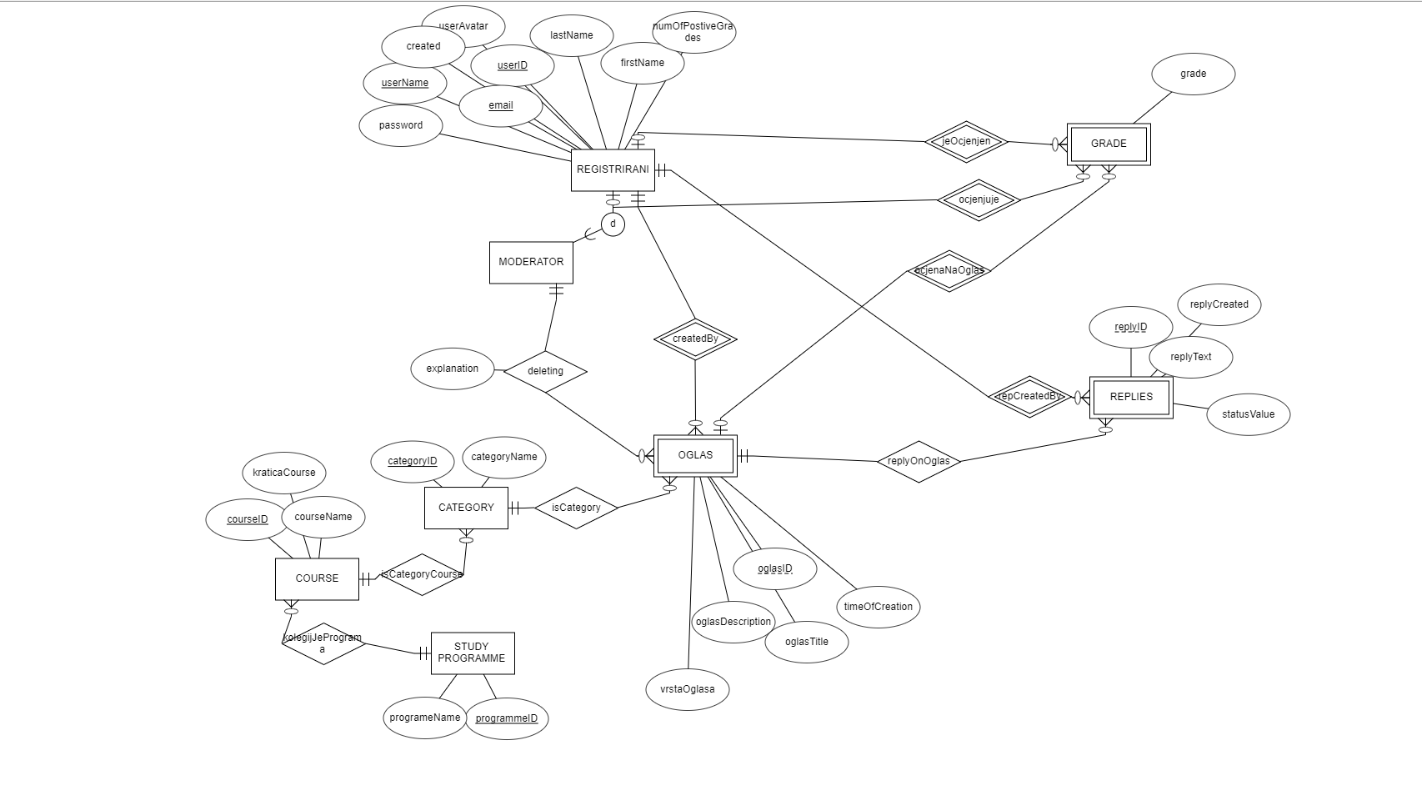
\includegraphics[width=\textwidth]{ER-dijagram Baze Podataka}
                \caption{\Slika 4.1: E-R dijagram baze podataka.}
			    
			\end{fig}

 
			
			\eject
			
			
		\section{Dijagram razreda}
		
			\textit{Potrebno je priložiti dijagram razreda s pripadajućim opisom. Zbog preglednosti je moguće dijagram razlomiti na više njih, ali moraju biti grupirani prema sličnim razinama apstrakcije i srodnim funkcionalnostima.}\\
			
			\textbf{\textit{dio 1. revizije}}\\
			
			\textit{Prilikom prve predaje projekta, potrebno je priložiti potpuno razrađen dijagram razreda vezan uz \textbf{generičku funkcionalnost} sustava. Ostale funkcionalnosti trebaju biti idejno razrađene u dijagramu sa sljedećim komponentama: nazivi razreda, nazivi metoda i vrste pristupa metodama (npr. javni, zaštićeni), nazivi atributa razreda, veze i odnosi između razreda.}\\
			
			\textbf{\textit{dio 2. revizije}}\\			
			
			\textit{Prilikom druge predaje projekta dijagram razreda i opisi moraju odgovarati stvarnom stanju implementacije}
			
			
			
			\eject
		
		\section{Dijagram stanja}
			
			
			\textbf{\textit{dio 2. revizije}}\\
			
			\textit{Potrebno je priložiti dijagram stanja i opisati ga. Dovoljan je jedan dijagram stanja koji prikazuje \textbf{značajan dio funkcionalnosti} sustava. Na primjer, stanja korisničkog sučelja i tijek korištenja neke ključne funkcionalnosti jesu značajan dio sustava, a registracija i prijava nisu. }
			
			
			\eject 
		
		\section{Dijagram aktivnosti}
			
			\textbf{\textit{dio 2. revizije}}\\
			
			 \textit{Potrebno je priložiti dijagram aktivnosti s pripadajućim opisom. Dijagram aktivnosti treba prikazivati značajan dio sustava.}
			
			\eject
		\section{Dijagram komponenti}
		
			\textbf{\textit{dio 2. revizije}}\\
		
			 \textit{Potrebno je priložiti dijagram komponenti s pripadajućim opisom. Dijagram komponenti treba prikazivati strukturu cijele aplikacije.}
	\chapter{Implementacija i korisničko sučelje}
		
		
		\section{Korištene tehnologije i alati}
		
			\textbf{\textit{dio 2. revizije}}
			
			 \textit{Detaljno navesti sve tehnologije i alate koji su primijenjeni pri izradi dokumentacije i aplikacije. Ukratko ih opisati, te navesti njihovo značenje i mjesto primjene. Za svaki navedeni alat i tehnologiju je potrebno \textbf{navesti internet poveznicu} gdje se mogu preuzeti ili više saznati o njima}.
			
			
			\eject 
		
	
		\section{Ispitivanje programskog rješenja}
			
			\textbf{\textit{dio 2. revizije}}\\
			
			 \textit{U ovom poglavlju je potrebno opisati provedbu ispitivanja implementiranih funkcionalnosti na razini komponenti i na razini cijelog sustava s prikazom odabranih ispitnih slučajeva. Studenti trebaju ispitati temeljnu funkcionalnost i rubne uvjete.}
	
			
			\subsection{Ispitivanje komponenti}
			\textit{Potrebno je provesti ispitivanje jedinica (engl. unit testing) nad razredima koji implementiraju temeljne funkcionalnosti. Razraditi \textbf{minimalno 6 ispitnih slučajeva} u kojima će se ispitati redovni slučajevi, rubni uvjeti te izazivanje pogreške (engl. exception throwing). Poželjno je stvoriti i ispitni slučaj koji koristi funkcionalnosti koje nisu implementirane. Potrebno je priložiti izvorni kôd svih ispitnih slučajeva te prikaz rezultata izvođenja ispita u razvojnom okruženju (prolaz/pad ispita). }
			
			
			
			\subsection{Ispitivanje sustava}
			
			 \textit{Potrebno je provesti i opisati ispitivanje sustava koristeći radni okvir Selenium\footnote{\url{https://www.seleniumhq.org/}}. Razraditi \textbf{minimalno 4 ispitna slučaja} u kojima će se ispitati redovni slučajevi, rubni uvjeti te poziv funkcionalnosti koja nije implementirana/izaziva pogrešku kako bi se vidjelo na koji način sustav reagira kada nešto nije u potpunosti ostvareno. Ispitni slučaj se treba sastojati od ulaza (npr. korisničko ime i lozinka), očekivanog izlaza ili rezultata, koraka ispitivanja i dobivenog izlaza ili rezultata.\\ }
			 
			 \textit{Izradu ispitnih slučajeva pomoću radnog okvira Selenium moguće je provesti pomoću jednog od sljedeća dva alata:}
			 \begin{itemize}
			 	\item \textit{dodatak za preglednik \textbf{Selenium IDE} - snimanje korisnikovih akcija radi automatskog ponavljanja ispita	}
			 	\item \textit{\textbf{Selenium WebDriver} - podrška za pisanje ispita u jezicima Java, C\#, PHP koristeći posebno programsko sučelje.}
			 \end{itemize}
		 	\textit{Detalji o korištenju alata Selenium bit će prikazani na posebnom predavanju tijekom semestra.}
			
			\eject 
		
		
		\section{Dijagram razmještaja}
			
			\textbf{\textit{dio 2. revizije}}
			
			 \textit{Potrebno je umetnuti \textbf{specifikacijski} dijagram razmještaja i opisati ga. Moguće je umjesto specifikacijskog dijagrama razmještaja umetnuti dijagram razmještaja instanci, pod uvjetom da taj dijagram bolje opisuje neki važniji dio sustava.}
			
			\eject 
		
		\section{Upute za puštanje u pogon}
		
			\textbf{\textit{dio 2. revizije}}\\
		
			 \textit{U ovom poglavlju potrebno je dati upute za puštanje u pogon (engl. deployment) ostvarene aplikacije. Na primjer, za web aplikacije, opisati postupak kojim se od izvornog kôda dolazi do potpuno postavljene baze podataka i poslužitelja koji odgovara na upite korisnika. Za mobilnu aplikaciju, postupak kojim se aplikacija izgradi, te postavi na neku od trgovina. Za stolnu (engl. desktop) aplikaciju, postupak kojim se aplikacija instalira na računalo. Ukoliko mobilne i stolne aplikacije komuniciraju s poslužiteljem i/ili bazom podataka, opisati i postupak njihovog postavljanja. Pri izradi uputa preporučuje se \textbf{naglasiti korake instalacije uporabom natuknica} te koristiti što je više moguće \textbf{slike ekrana} (engl. screenshots) kako bi upute bile jasne i jednostavne za slijediti.}
			
			
			 \textit{Dovršenu aplikaciju potrebno je pokrenuti na javno dostupnom poslužitelju. Studentima se preporuča korištenje neke od sljedećih besplatnih usluga: \href{https://aws.amazon.com/}{Amazon AWS}, \href{https://azure.microsoft.com/en-us/}{Microsoft Azure} ili \href{https://www.heroku.com/}{Heroku}. Mobilne aplikacije trebaju biti objavljene na F-Droid, Google Play ili Amazon App trgovini.}
			
			
			\eject 
	\chapter{Zaključak i budući rad}
		
		\textbf{\textit{dio 2. revizije}}\\
		
		 \textit{U ovom poglavlju potrebno je napisati osvrt na vrijeme izrade projektnog zadatka, koji su tehnički izazovi prepoznati, jesu li riješeni ili kako bi mogli biti riješeni, koja su znanja stečena pri izradi projekta, koja bi znanja bila posebno potrebna za brže i kvalitetnije ostvarenje projekta i koje bi bile perspektive za nastavak rada u projektnoj grupi.}
		
		 \textit{Potrebno je točno popisati funkcionalnosti koje nisu implementirane u ostvarenoj aplikaciji.}
		
		\eject 
	\chapter*{Popis literature}
		\addcontentsline{toc}{chapter}{Popis literature}
	 	
 		\textbf{\textit{Kontinuirano osvježavanje}}
	
		\textit{Popisati sve reference i literaturu koja je pomogla pri ostvarivanju projekta.}
		
		
		\begin{enumerate}
			
			
			\item  Programsko inženjerstvo, FER ZEMRIS, \url{http://www.fer.hr/predmet/proinz}
			
			\item  I. Sommerville, "Software engineering", 8th ed, Addison Wesley, 2007.
			
			\item  T.C.Lethbridge, R.Langaniere, "Object-Oriented Software Engineering", 2nd ed. McGraw-Hill, 2005.
			
			\item  I. Marsic, Software engineering book``, Department of Electrical and Computer Engineering, Rutgers University, \url{http://www.ece.rutgers.edu/~marsic/books/SE}
			
			\item  The Unified Modeling Language, \url{https://www.uml-diagrams.org/}
			
			\item  Astah Community, \url{http://astah.net/editions/uml-new}
		\end{enumerate}
		
		 
	
	
	\begingroup
	\renewcommand*\listfigurename{Indeks slika i dijagrama}
	%\renewcommand*\listtablename{Indeks tablica}
	%\let\clearpage\relax
	\listoffigures
	%\vspace{10mm}
	%\listoftables
	\endgroup
	\addcontentsline{toc}{chapter}{Indeks slika i dijagrama}


	
	\eject 
		
	\chapter*{Dodatak: Prikaz aktivnosti grupe}
		\addcontentsline{toc}{chapter}{Dodatak: Prikaz aktivnosti grupe}
		
		\section*{Dnevnik sastajanja}
		
		\textbf{\textit{Kontinuirano osvježavanje}}\\
		
		 \textit{U ovom dijelu potrebno je redovito osvježavati dnevnik sastajanja prema predlošku.}
		
		\begin{packed_enum}
			\item  sastanak
			
			\item[] \begin{packed_item}
				\item Datum: u ovom formatu: \today
				\item Prisustvovali: I.Prezime, I.Prezime
				\item Teme sastanka:
				\begin{packed_item}
					\item  opis prve teme
					\item  opis druge teme
				\end{packed_item}
			\end{packed_item}
			
			\item  sastanak
			\item[] \begin{packed_item}
				\item Datum: u ovom formatu: \today
				\item Prisustvovali: I.Prezime, I.Prezime
				\item Teme sastanka:
				\begin{packed_item}
					\item  opis prve teme
					\item  opis druge teme
				\end{packed_item}
			\end{packed_item}
			
			%
			
		\end{packed_enum}
		
		\eject
		\section*{Tablica aktivnosti}
		
			\textbf{\textit{Kontinuirano osvježavanje}}\\
			
			 \textit{Napomena: Doprinose u aktivnostima treba navesti u satima po članovima grupe po aktivnosti.}

			\begin{longtblr}[
					label=none,
				]{
					vlines,hlines,
					width = \textwidth,
					colspec={X[7, l]X[1, c]X[1, c]X[1, c]X[1, c]X[1, c]X[1, c]X[1, c]}, 
					vline{1} = {1}{text=\clap{}},
					hline{1} = {1}{text=\clap{}},
					rowhead = 1,
				} 
				\multicolumn{1}{c|}{} & \multicolumn{1}{c|}{\rotatebox{90}{\textbf{Ime Prezime voditelja}}} & \multicolumn{1}{c|}{\rotatebox{90}{\textbf{Ime Prezime }}} &	\multicolumn{1}{c|}{\rotatebox{90}{\textbf{Ime Prezime }}} & \multicolumn{1}{c|}{\rotatebox{90}{\textbf{Ime Prezime }}} &	\multicolumn{1}{c|}{\rotatebox{90}{\textbf{Ime Prezime }}} & \multicolumn{1}{c|}{\rotatebox{90}{\textbf{Ime Prezime }}} &	\multicolumn{1}{c|}{\rotatebox{90}{\textbf{Ime Prezime }}} \\  
				Upravljanje projektom 		&  &  &  &  &  &  & \\ 
				Opis projektnog zadatka 	&  &  &  &  &  &  & \\ 
				
				Funkcionalni zahtjevi       &  &  &  &  &  &  &  \\ 
				Opis pojedinih obrazaca 	&  &  &  &  &  &  &  \\ 
				Dijagram obrazaca 			&  &  &  &  &  &  &  \\ 
				Sekvencijski dijagrami 		&  &  &  &  &  &  &  \\ 
				Opis ostalih zahtjeva 		&  &  &  &  &  &  &  \\ 

				Arhitektura i dizajn sustava	 &  &  &  &  &  &  &  \\ 
				Baza podataka				&  &  &  &  &  &  &   \\ 
				Dijagram razreda 			&  &  &  &  &  &  &   \\ 
				Dijagram stanja				&  &  &  &  &  &  &  \\ 
				Dijagram aktivnosti 		&  &  &  &  &  &  &  \\ 
				Dijagram komponenti			&  &  &  &  &  &  &  \\ 
				Korištene tehnologije i alati 		&  &  &  &  &  &  &  \\ 
				Ispitivanje programskog rješenja 	&  &  &  &  &  &  &  \\ 
				Dijagram razmještaja			&  &  &  &  &  &  &  \\ 
				Upute za puštanje u pogon 		&  &  &  &  &  &  &  \\  
				Dnevnik sastajanja 			&  &  &  &  &  &  &  \\ 
				Zaključak i budući rad 		&  &  &  &  &  &  &  \\  
				Popis literature 			&  &  &  &  &  &  &  \\  
				&  &  &  &  &  &  &  \\ \hline 
				\textit{Dodatne stavke kako ste podijelili izradu aplikacije} 			&  &  &  &  &  &  &  \\ 
				\textit{npr. izrada početne stranice} 				&  &  &  &  &  &  &  \\  
				\textit{izrada baze podataka} 		 			&  &  &  &  &  &  & \\  
				\textit{spajanje s bazom podataka} 							&  &  &  &  &  &  &  \\ 
				\textit{back end} 							&  &  &  &  &  &  &  \\  
				 							&  &  &  &  &  &  &\\ 
			\end{longtblr}
					
					
		\eject
		\section*{Dijagrami pregleda promjena}
		
		\textbf{\textit{dio 2. revizije}}\\
		
		\textit{Prenijeti dijagram pregleda promjena nad datotekama projekta. Potrebno je na kraju projekta generirane grafove s gitlaba prenijeti u ovo poglavlje dokumentacije. Dijagrami za vlastiti projekt se mogu preuzeti s gitlab.com stranice, u izborniku Repository, pritiskom na stavku Contributors.}
		
	


\end{document} %naredbe i tekst nakon ove naredbe ne ulaze u izgrađen dokument 


